\newpage
\subsection{filter}
In this context, filtering is defined as checking whether single hits or events holds a certain quantitative condition or criterium. No data is thrown out. Thus, the output array of a filter contains boolean (values are 'true' or 'false'). An example of an input signal filter, its input and output matrix, is given in the following table.

\begin{table}
\center
\caption{Input and output array for a filter only approving input values between and including 4 to 9. ($4 \leq x \leq 9$)}
\begin{tabular}{cc}
input array 	& output array\\
\hline
3				& false\\
4				& true\\
7				& true\\
2 				& false\\
12				& false\\
8				& true\\
1 				& false\\
\end{tabular}
\end{table}

combining multiple filters can be done in a single line.
\begin{itemize}
\item \emph{filter\_array\_3  = filter\_array\_1 \&\& filter\_array\_2} if both filter conditions should hold
\item \emph{filter\_array\_3  = filter\_array\_1 \textbar\textbar filter\_array\_2} if either condition should hold.
\end{itemize}

Filtering can be done on the events and on the hits. An example of a filter on events is the filtering of all double coincidence events. An example for hits is a TOF that filters out a certain chemical mass. When a set of hits is filtered, the corresponding hits can be identified and thus a event-based filter array can be built. This can be done with function XXXX. This can be needed when a certain condition is imposed on one detector, and the user wants to visualize the remaining events on another detector.

The filtering arrays are stored under the name \emph{filter\_h\_}*name* for events, and \emph{filter\_h\_}*det\_name* \_ *name* for hits. For the hit filter arrays, the detector name needs to be specified, since hits among different detectors need not be correlated. 


\begin{figure}[h]
   \centering
    \centerline{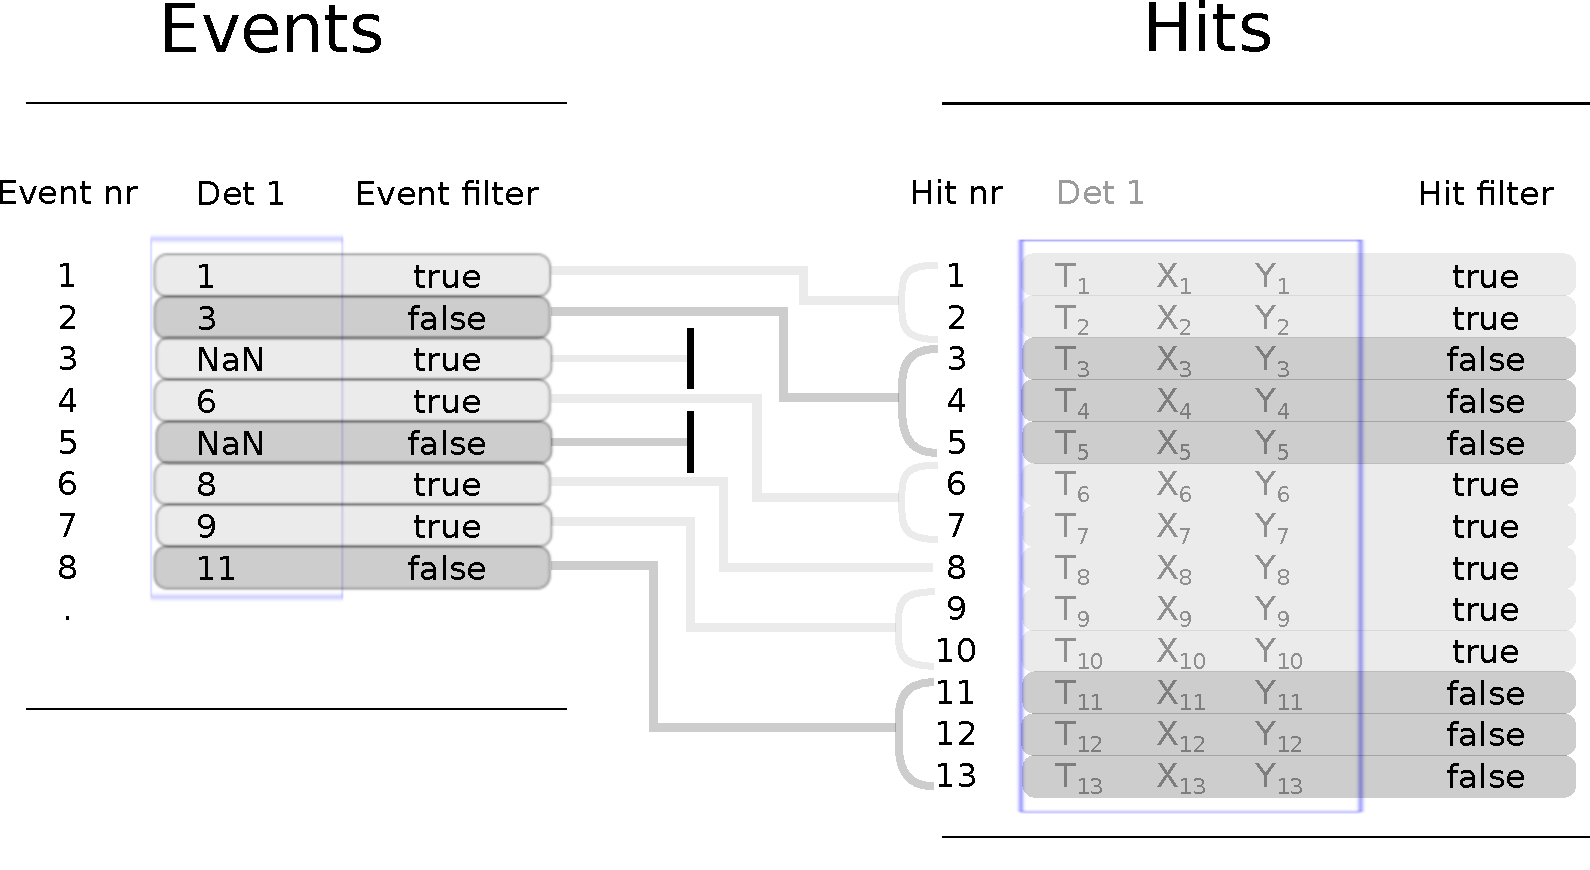
\includegraphics[width=0.9\textwidth]{Graphics/Filter_event2hit.pdf}}
\caption{The translation of an example event filter to a hit filter.}
\label{Data_structure_schematic}
\end{figure}

\begin{figure}[h]
   \centering
    \centerline{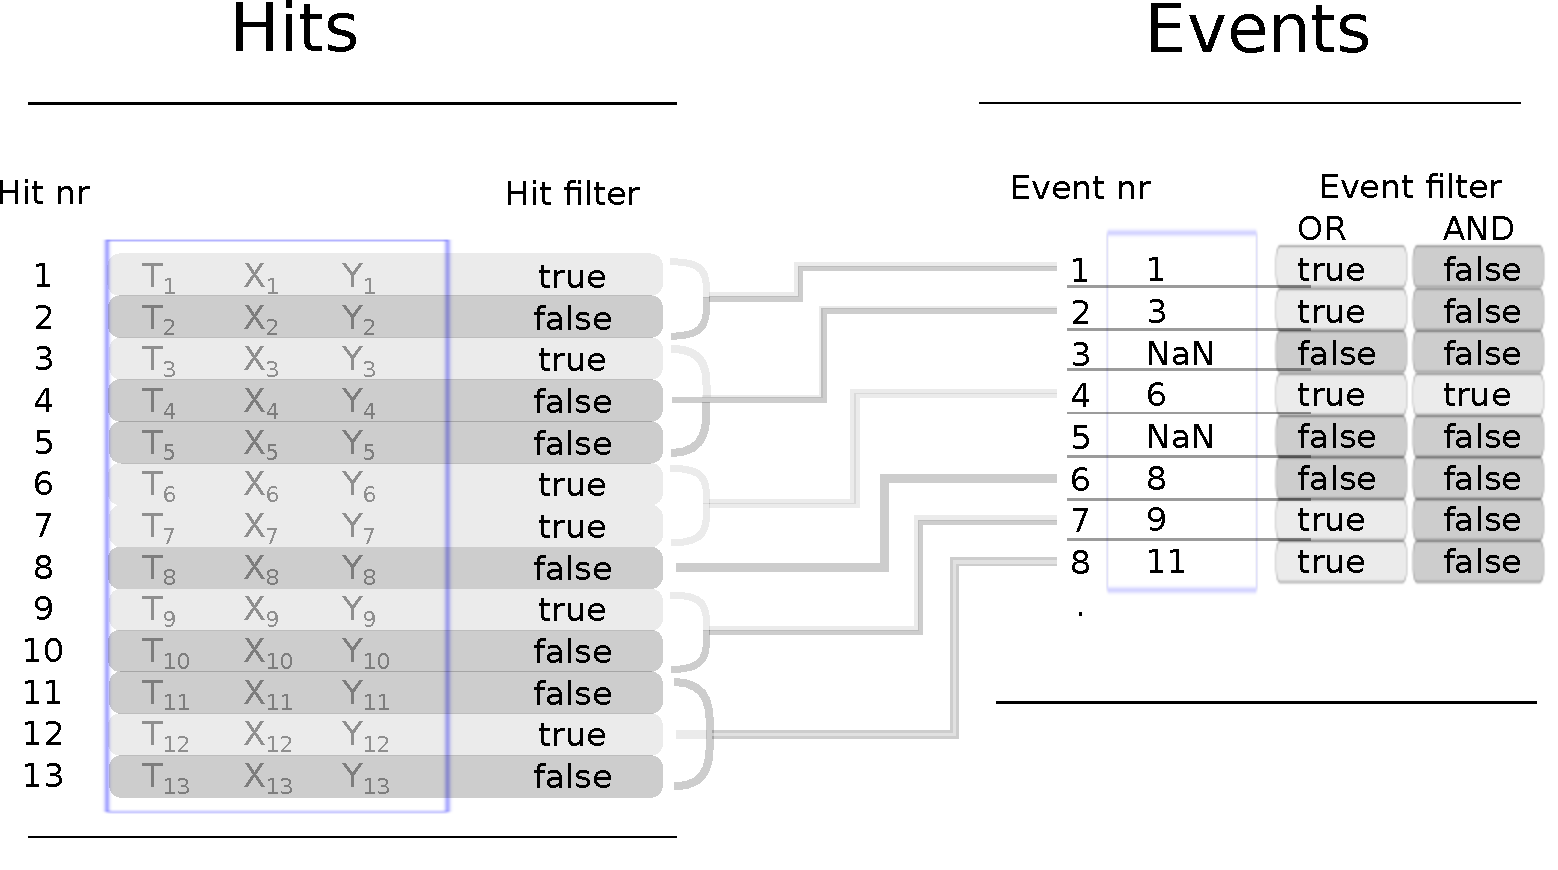
\includegraphics[width=0.9\textwidth]{Graphics/Filter_hit2event.pdf}}
\caption{The translation of an example hit filter to an event filter.}
\label{Data_structure_schematic}
\end{figure}

